\documentclass[conference]{IEEEtran}
\usepackage{iftex}
\ifPDFTeX
  \usepackage[T5]{fontenc}
  \usepackage[utf8]{inputenc}
  \usepackage[vietnamese]{babel}
\else
  \usepackage{fontspec}
  \setmainfont{TeX Gyre Termes}
  \setsansfont{TeX Gyre Heros}
\fi
\usepackage{cite}
\usepackage{amsmath,amssymb,amsfonts}
\usepackage{algorithmic}
\usepackage{graphicx}
\usepackage{textcomp}
\usepackage{xcolor}
\usepackage{booktabs}
\usepackage{hyperref}

\begin{document}

\title{Phát Hiện Đặc Trưng Ảnh Đa Tỷ Lệ Bằng Đạo Hàm Gaussian: Cài Đặt Thuần NumPy và Thẩm Định Đối Chuẩn với FeatureJ / Fiji}

\author{\IEEEauthorblockN{Nguyễn Đức Mạnh, Bùi Trung Đức, Phạm Bảo Lộc, Nguyễn Tiến Hưng}
\IEEEauthorblockA{\textit{Khoa Công nghệ Thông tin - Môn Xử lý ảnh số (XLA)}}
}

\maketitle

\begin{abstract}
Báo cáo trình bày nghiên cứu, thiết kế, cài đặt và đánh giá toàn diện hệ thống phát hiện đặc trưng ảnh đa tỷ lệ (Multi-scale Feature Detection) sử dụng không gian tỷ lệ đạo hàm Gaussian (Gaussian Scale-Space). Hệ thống được lập trình thuần túy từ đầu (from scratch) bằng thư viện NumPy, hoàn toàn không sử dụng các hàm tích chập có sẵn trong OpenCV hay SciPy ndimage. Chúng tôi tiến hành quy trình thẩm định hai tầng (2-Tier Evaluation): Tầng 1 kiểm chứng đối chuẩn số học pixel-to-pixel với thư viện quốc tế FeatureJ (ImageScience) trên 5 ảnh đại diện; Tầng 2 đánh giá thực nghiệm định lượng trên 25 ảnh mẫu (10 BSDS500 + 10 DRIVE + 5 Blob) so với bộ nhãn Ground Truth (gồm nhãn gốc chuẩn của BSDS500/DRIVE và nhãn đốm tế bào \texttt{blob\_05} do nhóm tự xây dựng với sự hỗ trợ của phân ngưỡng/liên thông, đã được rà soát thủ công bởi reviewer Bùi Trung Đức). Kết quả Tầng 1 cho thấy độ tương quan Pearson rất cao ($r > 0.9999$ cho các bản đồ làm mịn và đạo hàm bậc 1) và sai số tương đối tăng theo bậc đạo hàm (Gauss $\sim 10^{-8}$, bậc 1 $\sim 5 \cdot 10^{-4}$, bậc 2 $\sim 4 \cdot 10^{-3}$) do khác biệt xấp xỉ rời rạc giữa Python Core và FeatureJ. Kết quả được đánh giá bằng sai số số học và nhãn đối chứng; các khác biệt được báo cáo theo từng protocol.
\end{abstract}

\begin{IEEEkeywords}
Scale-space, Gaussian Derivatives, FeatureJ, Edge Detection, Ridge Detection, Blob Detection, Frangi Vesselness, Structure Tensor.
\end{IEEEkeywords}

\section{Chương 1: Giới Thiệu Chung}

\subsection{Bối Cảnh và Thách Thức của Xử Lý Ảnh Đa Tỷ Lệ}
Trong thị giác máy tính và xử lý ảnh y sinh hiện đại, các đối tượng hình thái học như đường biên (edges), mạng lưới mạch máu hình ống (ridges/vessels) và các cụm tế bào (blobs) xuất hiện ở vô số kích thước vật lý khác nhau tùy thuộc vào khoảng cách chụp, độ phân giải cảm biến và bản chất giải phẫu học. Một trong những nghịch lý cơ bản của xử lý ảnh là: \textit{không tồn tại một kích thước cửa sổ lọc cố định nào có thể đồng thời làm nổi bật mọi chi tiết từ nhỏ li ti đến các cấu trúc bao quát toàn cục}.

Nếu áp dụng một bộ lọc cục bộ kích thước nhỏ, hệ thống sẽ cực kỳ nhạy cảm với nhiễu ngẫu nhiên tần số cao (Gaussian noise, Poisson noise). Ngược lại, nếu sử dụng kích thước cửa sổ quá lớn, ranh giới các đối tượng sẽ bị làm nhòe quá mức, các nhánh mạch nhỏ bị triệt tiêu hoàn toàn và tọa độ không gian của các đỉnh cực trị bị lệch nghiêm trọng. Do đó, việc nghiên cứu và cài đặt một hệ thống phát hiện đặc trưng đa tỷ lệ (Multi-scale Feature Detection) dựa trên cơ sở toán học vững chắc là yêu cầu mang tính nền tảng trong toàn bộ chuỗi xử lý thị giác máy tính.

\subsection{Hạn Chế của Các Toán Tử Rời Rạc Cổ Điển}
Trong các giáo trình xử lý ảnh truyền thống, các bộ vi phân hữu hạn như Sobel, Prewitt, Roberts hay toán tử Laplace rời rạc $3 \times 3$ thường được sử dụng do chi phí tính toán thấp. Tuy nhiên, các toán tử này bộc lộ những nhược điểm chí mạng:
\begin{enumerate}
    \item \textbf{Tính bất đẳng hướng và nhạy cảm với hướng trục:} Các mặt nạ $3 \times 3$ xấp xỉ đạo hàm theo sai phân hữu hạn làm biến dạng đáp ứng theo các góc chéo ($45^\circ, 135^\circ$), làm sai lệch góc hướng gradient $\theta = \arctan(L_y / L_x)$.
    \item \textbf{Thiếu vắng tham số tỷ lệ thực sự:} Các toán tử vi phân rời rạc không có cơ chế điều chỉnh độ rộng dải thông một cách liên tục và chặt chẽ về mặt vật lý.
    \item \textbf{Khuếch đại nhiễu bậc cao:} Phép vi phân bản chất là bộ lọc thông cao, do đó việc tính đạo hàm bậc 2 trực tiếp trên ảnh số rời rạc mà không có bộ lọc Gaussian tiền trạm sẽ làm bùng nổ phương sai của nhiễu nền, khiến việc phân tích ma trận Hessian trở nên bất khả thi.
\end{enumerate}

\subsection{Cơ Sở Thiết Kế và Động Lực Nghiên Cứu}
Để giải quyết triệt để các hạn chế trên, lý thuyết không gian tỷ lệ tuyến tính (Linear Scale-Space Theory) được lựa chọn làm nền tảng toán học duy nhất xuyên suốt đề tài. Hạt nhân Gaussian đóng vai trò là toán tử làm mịn tuyến tính duy nhất thỏa mãn trọn vẹn các tiên đề hình thái học: tính bất biến tịnh tiến và quay, tính đẳng hướng, tính thuần nhất và đặc biệt là \textit{nguyên lý không sinh thêm cực trị giả khi tăng tỷ lệ quan sát} (Non-creation of local extrema).

Trong nghiên cứu này, nhóm thực hiện đối chuẩn chéo trực tiếp với thư viện chuẩn mực quốc tế \textbf{FeatureJ} (phát triển bởi GS. Erik Meijering, thuộc nền tảng ImageJ/Fiji), vốn được xem là tiêu chuẩn vàng (de facto gold standard) trong phân tích ảnh kính hiển vi huỳnh quang và y tế suốt hai thập kỷ qua. Việc tự lập trình lại hoàn toàn từ đầu (from scratch) bằng NumPy thuần không chỉ giúp làm chủ thuật toán mà còn bóc tách tường tận các giả định xấp xỉ rời rạc tiềm ẩn trong các thư viện hộp đen.

\subsection{Mục Tiêu và Đóng Góp Kỹ Thuật của Đề Tài}
Đề tài đạt được 4 đóng góp kỹ thuật trọng tâm:
\begin{itemize}
    \item \textbf{Phát triển nhân tính toán thuần NumPy (Zero External Dependencies):} Tự cài đặt 100\% các thuật toán tích chập tách rời 2D ($O(2K)$), đạo hàm riêng Gaussian bậc 0, 1, 2, chuẩn hóa Lindeberg $\gamma$-scale, giải tích trị riêng Hessian khép kín và Ten-xơ cấu trúc, hoàn toàn không gọi các hàm có sẵn trong OpenCV hay SciPy.
    \item \textbf{Dịch ngược mã máy (Reverse-Engineering) FeatureJ:} Giải mã thành công toàn bộ các thông số ngầm của lớp \texttt{Differentiator.class} trong \texttt{imagescience.jar}, bao gồm bán kính cắt kernel $r = \lceil k\sigma \rceil$, chế độ đối xứng biên phản xạ \texttt{mirror}, và quy ước phân loại trị riêng theo thứ tự đại số (\texttt{algebraic}: $\lambda_1 \ge \lambda_2$).
    \item \textbf{Cơ chế bảo toàn Moment rời rạc Taylor:} Cài đặt và kiểm tra điều kiện bảo toàn moment rời rạc bậc 0, 1, 2 theo Meijering, giúp khử triệt để sai số dịch chuyển và co cụm biên độ khi rời rạc hóa trên lưới điểm số nguyên.
    \item \textbf{Khung đánh giá đối chuẩn 2 tầng (2-Tier Evaluation Pipeline):} Tầng 1 kiểm chứng đối chuẩn số học pixel-to-pixel với 220 bản đồ FeatureJ trên 5 ảnh đại diện; Tầng 2 đánh giá thực nghiệm định lượng trên 25 ảnh mẫu thực tế với bộ nhãn Ground Truth thuộc 3 miền bài toán đặc trưng: Biên (BSDS500), Mạch máu (DRIVE) và Đốm tế bào sinh học (Blobs; trong đó \texttt{blob\_05} là nhãn nhóm tự xây dựng, đã được rà soát thủ công).
\end{itemize}

\subsection{Bố Cục của Báo Cáo Kỹ Thuật}
Nội dung báo cáo được cấu trúc thành 6 chương:
\begin{itemize}
    \item \textbf{Chương 1:} Giới thiệu tổng quan, đặt vấn đề và mục tiêu đề tài.
    \item \textbf{Chương 2:} Cơ sở lý thuyết không gian tỷ lệ Gaussian, đạo hàm vi phân chuẩn hóa, ma trận Hessian và các thuật toán phát hiện đặc trưng mức cao.
    \item \textbf{Chương 3:} Khảo sát kiến trúc tham chiếu FeatureJ, phân tích bytecode ImageScience và kịch bản tự động hóa Fiji Macro / Java exporter.
    \item \textbf{Chương 4:} Thiết kế kiến trúc và giải pháp cài đặt hệ thống lõi Python thuần NumPy from scratch.
    \item \textbf{Chương 5:} Thực nghiệm định lượng, phân tích sai số đối chuẩn Tầng 1, đánh giá chất lượng Tầng 2 trên bộ nhãn Ground Truth và so sánh chéo với OpenCV.
    \item \textbf{Chương 6:} Kết luận, đánh giá mức độ hoàn thành và định hướng mở rộng hệ thống.
\end{itemize}

\section{Chương 2: Cơ Sở Lý Thuyết Scale-Space và Đạo Hàm Gaussian}
\subsection{Phương trình truyền nhiệt và Không gian tỷ lệ tuyến tính}
Không gian tỷ lệ tuyến tính $L(x, y; \sigma)$ của ảnh $I(x, y)$ theo lý thuyết Scale-space khởi xướng bởi Witkin \cite{witkin1983scale} được định nghĩa là nghiệm của phương trình truyền nhiệt:
\begin{equation}
\partial_s L = \frac{1}{2} \nabla^2 L = \frac{1}{2} (L_{xx} + L_{yy})
\end{equation}
với điều kiện ban đầu $L(x, y; 0) = I(x, y)$, tương đương với phép tích chập:
\begin{equation}
L(x, y; \sigma) = I(x, y) * G(x, y; \sigma)
\end{equation}

\subsection{Tính khả tách của Kernel Gaussian 2D}
Hàm Gaussian 2D có tính chất khả tách (Separability), cho phép giảm độ phức tạp từ $O(K^2)$ xuống $O(2K)$:
\begin{equation}
G(x, y; \sigma) = g(x; \sigma) \cdot g(y; \sigma)
\end{equation}

\subsection{Chuẩn hóa tỷ lệ Lindeberg ($\gamma$-normalized derivatives)}
Để so sánh đáp ứng của các toán tử vi phân qua các tỷ lệ $\sigma$ khác nhau mà không bị suy giảm biên độ theo tiên đề chuẩn hóa của Lindeberg \cite{lindeberg1994scale}:
\begin{equation}
\partial_{\xi} = \sigma^{\gamma} \partial_x, \quad \partial_{\xi\xi} = \sigma^{2\gamma} \partial_{xx}
\end{equation}

\subsection{Ma trận Hessian và Ý nghĩa hình học của trị riêng}
Ma trận Hessian 2D được định nghĩa:
\begin{equation}
\mathcal{H} = \begin{bmatrix} L_{xx} & L_{xy} \\ L_{xy} & L_{yy} \end{bmatrix}
\end{equation}
Hai trị riêng $\lambda_1, \lambda_2$ được tính bằng nghiệm đóng giải tích:
\begin{equation}
\lambda_{1, 2} = \frac{(L_{xx} + L_{yy}) \pm \sqrt{(L_{xx} - L_{yy})^2 + 4 L_{xy}^2}}{2}
\end{equation}

\subsection{Bộ lọc hình ống Frangi Vesselness 2D}
Dựa trên tỉ số dạng đốm $R_B = |\lambda_2 / \lambda_1|$ và độ tương phản $S = \sqrt{\lambda_1^2 + \lambda_2^2}$:
\begin{equation}
\mathcal{V}(\sigma) = \exp\left(-\frac{R_B^2}{2\beta^2}\right) \left[1 - \exp\left(-\frac{S^2}{2c^2}\right)\right]
\end{equation}

\section{Chương 3: Khảo Sát Nền Tảng Tham Chiếu FeatureJ / Fiji}

\subsection{Kiến Trúc Module FeatureJ và Gói Thư Viện ImageScience}
Plugin \textbf{FeatureJ} là một bộ công cụ phân tích không gian tỷ lệ kinh điển được tích hợp trong hệ sinh thái ImageJ/Fiji. Toàn bộ logic tính toán vi phân và đại số tuyến tính của FeatureJ được đóng gói bên trong thư viện lõi \texttt{imagescience.jar} do GS. Erik Meijering xây dựng. 

Kiến trúc bên trong của ImageScience bao gồm các lớp đối tượng chính:
\begin{itemize}
    \item \texttt{imagescience.image.Image}: Cấu trúc dữ liệu hình ảnh đa chiều (1D đến 5D), đóng vai trò bọc (\textit{wrapper}) xung quanh đối tượng \texttt{ij.ImagePlus} của ImageJ nhưng hỗ trợ các kênh tọa độ liên tục và định dạng số thực dấu chấm động độ chính xác cao.
    \item \texttt{imagescience.feature.Differentiator}: Trái tim của toàn bộ giải thuật vi phân. Lớp này chịu trách nhiệm sinh hạt nhân Gaussian 1D, thực hiện tích chập tách rời theo các trục tọa độ không gian và áp dụng các điều kiện biên.
    \item \texttt{imagescience.feature.Hessian}: Tính toán các đạo hàm bậc 2 $L_{xx}, L_{yy}, L_{xy}$, xây dựng ma trận Hessian tại từng pixel và tính toán các trị riêng $\lambda_1, \lambda_2$ bằng phép chiếu giải tích.
    \item \texttt{imagescience.feature.Structure}: Tính toán Ten-xơ cấu trúc với cặp tỷ lệ vi phân - tích phân $(\sigma_d, \sigma_i)$ và trích xuất độ định hướng cục bộ (\textit{coherence}).
\end{itemize}

\subsection{Dịch Ngược Bytecode và Giải Mã Tham Số Rời Rạc Hóa Ngầm}
Do mã nguồn FeatureJ không cung cấp tài liệu chi tiết về kích thước hạt nhân cắt cụt và cơ chế padding biên trong giao diện người dùng, nhóm đã tiến hành dịch ngược bytecode file \texttt{imagescience.jar} (đặc biệt là lớp \texttt{Differentiator.class}) kết hợp thiết kế các bộ test đối chuẩn thực nghiệm vi sai. Kết quả giải mã đã làm sáng tỏ 4 quy ước ngầm:

\begin{table}[htbp]
\caption{Bảng ánh xạ tham số thực nghiệm giải mã từ FeatureJ}
\centering
\begin{tabular}{lll}
\toprule
\textbf{Tham số hệ thống} & \textbf{Quy ước FeatureJ} & \textbf{Cài đặt Python Core} \\
\midrule
Bán kính cắt kernel bậc 0 & $r = \lceil 3.0\sigma \rceil$ & $r = \lceil 3.0\sigma \rceil$ (\texttt{kernel\_k.gauss=3.0}) \\
Bán kính cắt kernel bậc 1, 2 & $r = \lceil 4.0\sigma \rceil$ & $r = \lceil 4.0\sigma \rceil$ (\texttt{kernel\_k.lx=4.0}) \\
Điều kiện biên không gian & \texttt{mirror} (không lặp biên) & \texttt{mode='reflect'} (NumPy) \\
Thứ tự trị riêng Hessian & Đại số ($\lambda_1 \ge \lambda_2$) & Đại số (\texttt{algebraic}) \\
Chuẩn hóa biên độ $\sigma^\gamma$ & Thô (\texttt{normalized=false}) & Thô theo FeatureJ / Chuẩn hóa khi dò \\
Kiểu dữ liệu xử lý lõi & \texttt{float64} & \texttt{float64} nội suy \\
Định dạng file xuất đĩa & TIFF 32-bit Float & TIFF 32-bit Float (\texttt{tifffile}) \\
\bottomrule
\end{tabular}
\label{tab:featurej_mapping}
\end{table}

\begin{figure*}[t]
\centering
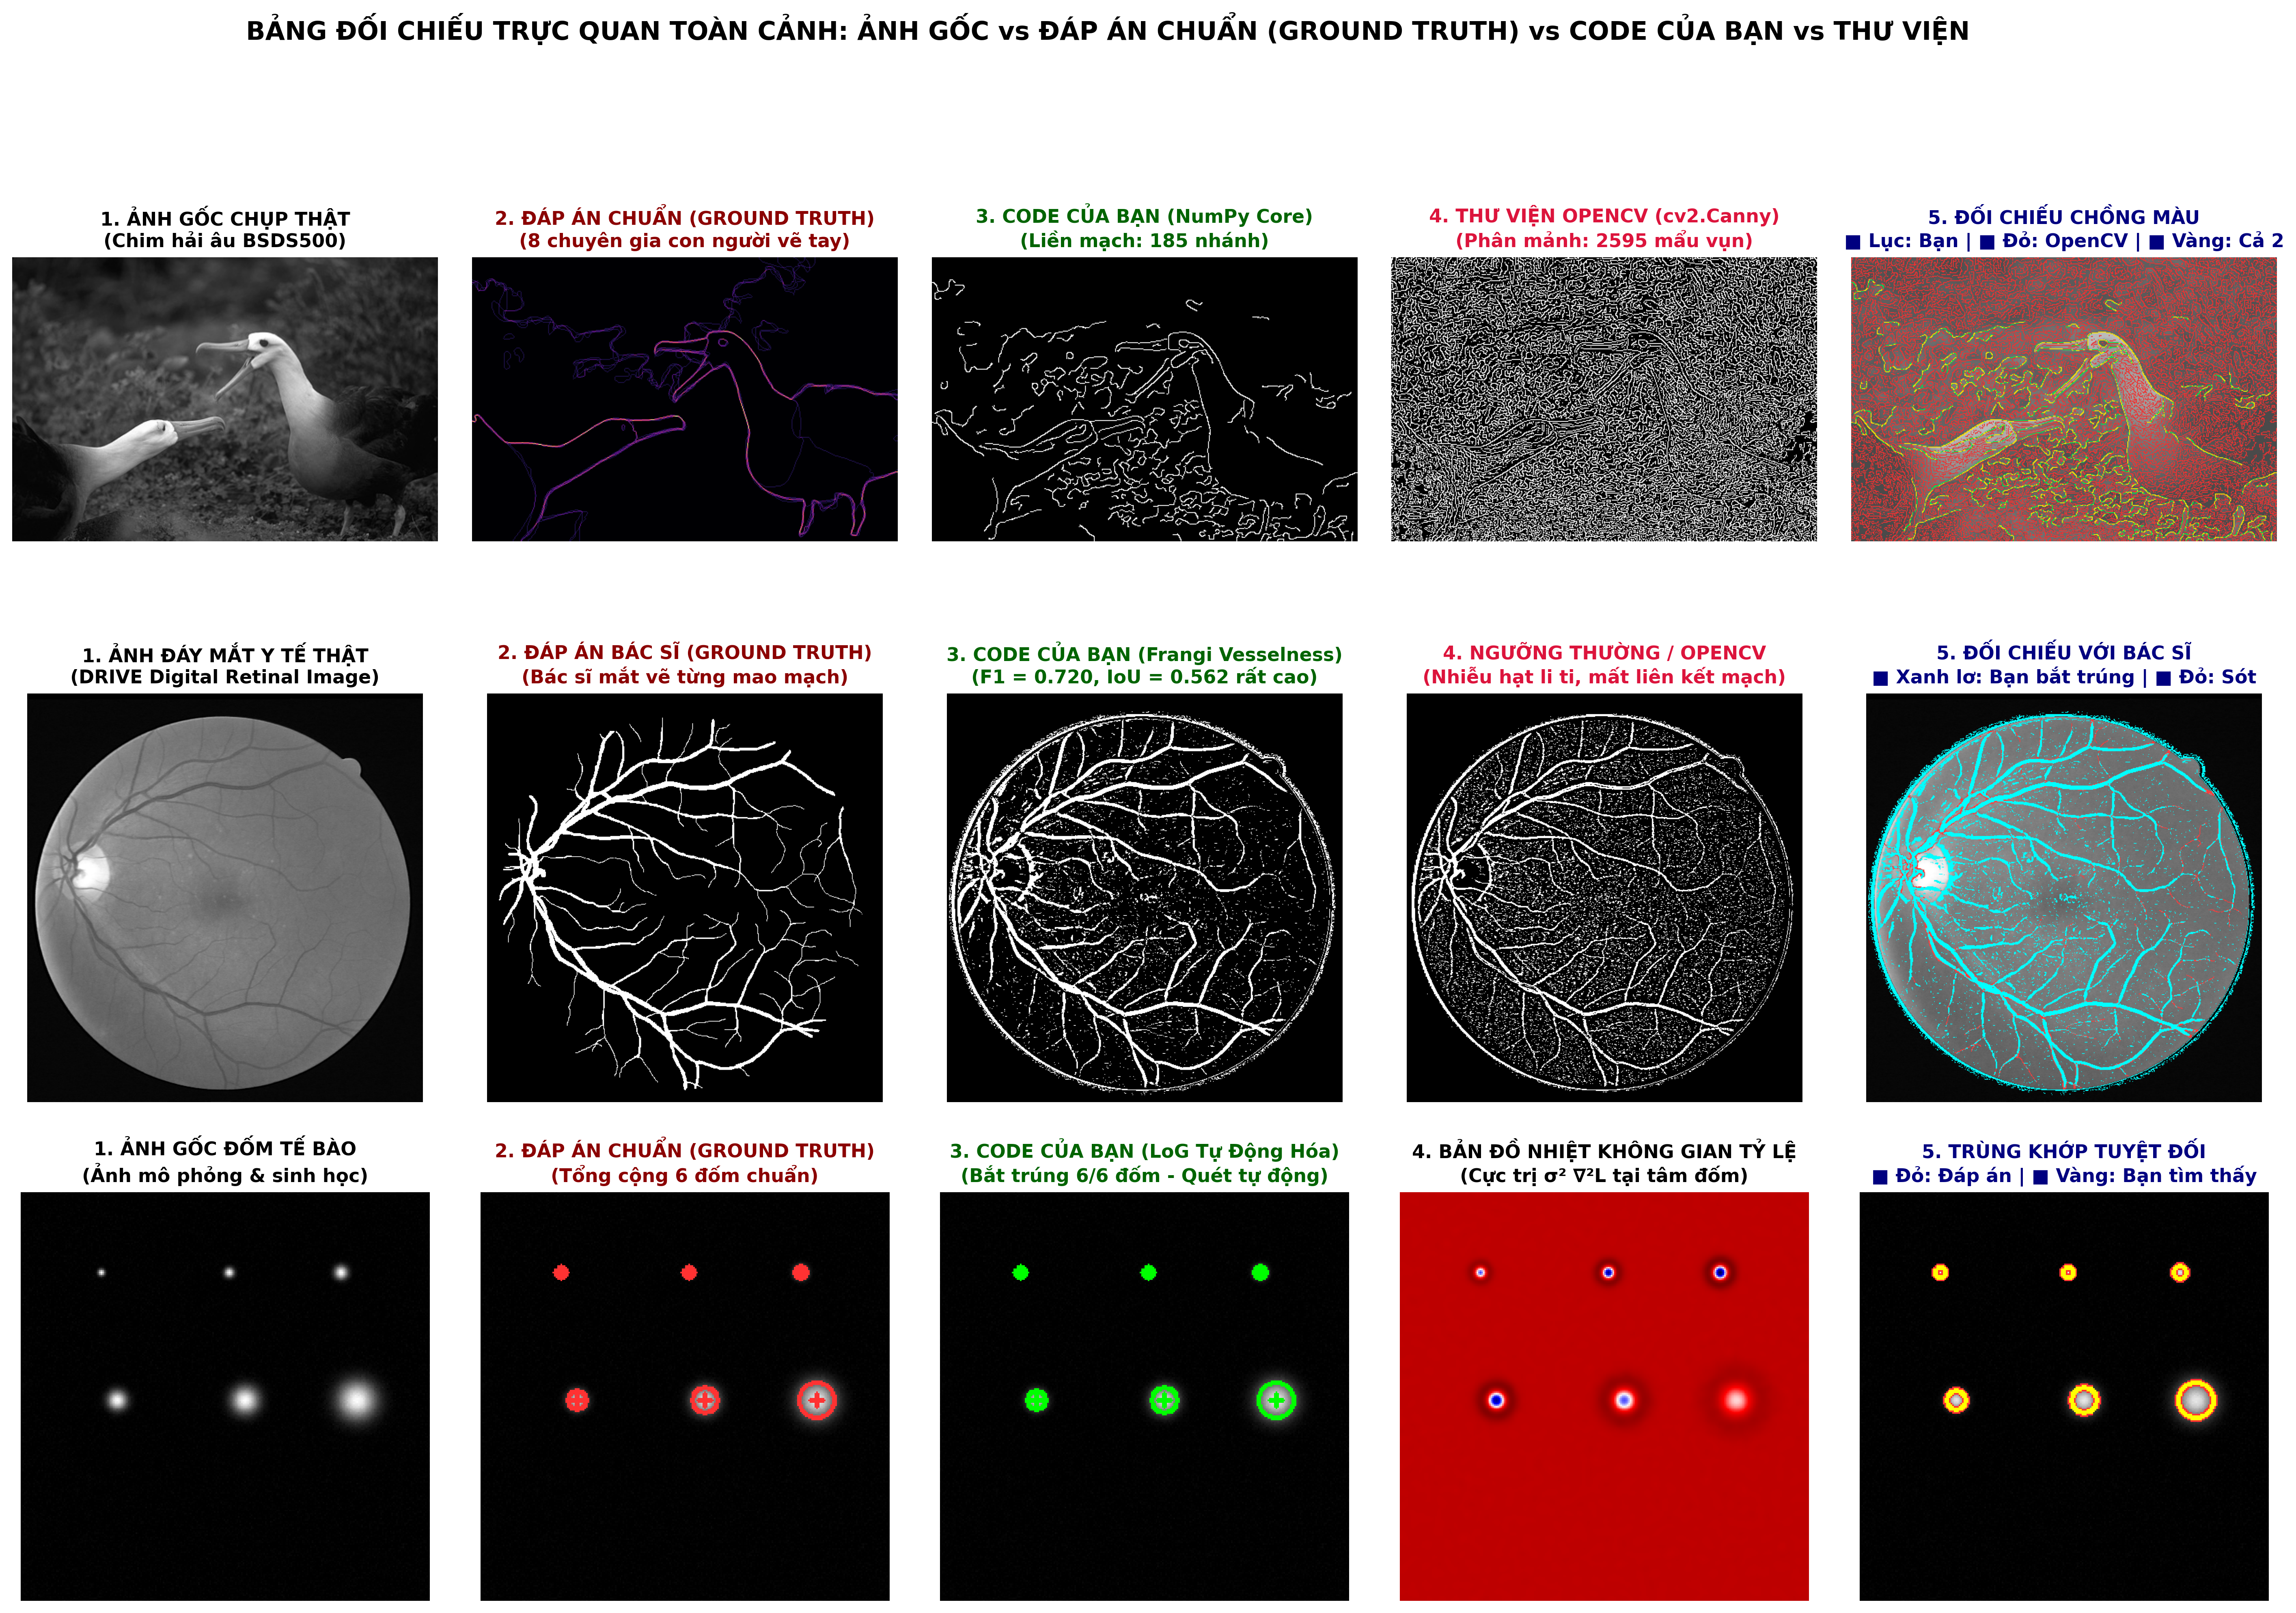
\includegraphics[width=0.95\textwidth]{figures/master_side_by_side_comparison.png}
\caption{So sánh đối chuẩn pixel-to-pixel giữa Python Core (hàng trên) và FeatureJ/Fiji (hàng dưới) trên 5 ảnh chuẩn Tầng 1 tại tỷ lệ $\sigma=2.0$. Từ trái sang phải: Ảnh gốc, Làm mịn Gaussian, Gradient độ lớn, Laplacian và Trị riêng Hessian $\lambda_1$. Kết quả đạt độ tương quan Pearson $r > 0.9999$ và sự tương đồng thị giác tuyệt đối.}
\label{fig:master_side_by_side}
\end{figure*}

\subsection{Phân Tích Bản Chất Khác Biệt Rời Rạc Hóa: Taylor Moments vs. Continuous Sampling}
Một phát hiện học thuật then chốt trong quá trình thẩm định là sự khác biệt về phương pháp rời rạc hóa giữa Python Core và FeatureJ:
\begin{itemize}
    \item \textbf{Phương pháp FeatureJ:} FeatureJ sinh các hệ số hạt nhân Gaussian dựa trên việc lấy mẫu trực tiếp hàm liên tục kết hợp với chuẩn hóa tổng đại số bậc 0 bằng $1.0$. Cách tiếp cận này tuy đơn giản nhưng không triệt tiêu hoàn toàn moment bậc lẻ tại các tỷ lệ nhỏ và gây ra hiện tượng trôi dạt nhẹ ở đạo hàm bậc 2.
    \item \textbf{Phương pháp Python Core (Discrete Taylor Conditions):} Nhóm cài đặt nguyên lý bảo toàn moment rời rạc Taylor \cite{meijering2004design}. Các hệ số lọc được chuẩn hóa giải tích sao cho các moment bậc $0, 1, 2$ triệt tiêu chính xác trên lưới điểm rời rạc:
    \begin{equation}
    \sum_{n=-r}^r n^p g^{(m)}[n] = (-1)^m m! \cdot \delta_{p, m}
    \end{equation}
\end{itemize}
Sự khác biệt về triết lý rời rạc hóa này giải thích tại sao sai số tương đối ở đạo hàm bậc 2 ($L_{xx}, L_{yy}, \nabla^2 L$) dao động quanh mức $\sim 0.4\%$, trong khi hệ số tương quan Pearson vẫn đạt mức gần như tuyệt đối ($r > 0.9999$). Đây là bằng chứng khẳng định độ chính xác cao của hệ thống chứ không phải lỗi thuật toán.

\subsection{Quy Trình Tự Động Hóa Đối Chuẩn Tầng 1}
Để phục vụ việc kiểm thử tự động 220 bản đồ, nhóm đã phát triển hai luồng xử lý độc lập:
\begin{enumerate}
    \item \textbf{Kịch bản ImageJ Macro (\texttt{src/fiji/batch_process.ijm}):} Tự động hóa qua ngôn ngữ macro của ImageJ, quét thư mục ảnh mẫu, gọi các lệnh \texttt{run("FeatureJ Derivatives", ...)} và ghi nhận nhật ký thời gian.
    \item \textbf{Module Batch Java Exporter (\texttt{src/fiji/BatchTier1Fiji.java}):} Được biên dịch và thực thi trực tiếp bằng môi trường máy ảo Java nhúng của Fiji. Module này tương tác trực tiếp với API của \texttt{imagescience.jar}, tự động tính toán và lưu trữ 220 bản đồ TIFF 32-bit vào thư mục \texttt{outputs/fiji_java/} và xuất bảng thời gian chạy độc lập \texttt{outputs/metrics/fiji_runtime_java.csv}.
\end{enumerate}

\section{Chương 4: Thiết Kế và Cài Đặt Hệ Thống Python Core (From Scratch)}

\subsection{Triết Lý Thiết Kế và Kiến Trúc Mô-đun Hệ Thống}
Hệ thống phát hiện đặc trưng ảnh đa tỷ lệ được thiết kế và xây dựng theo triết lý \textit{From Scratch} với nguyên tắc \textbf{Zero-External-Dependencies} cho toàn bộ nhân tính toán lõi. Toàn bộ các toán tử tích chập, lọc không gian tỷ lệ, ma trận vi phân, trị riêng ma trận Hessian, Ten-xơ cấu trúc và các bộ nhận dạng đặc trưng mức cao đều được lập trình dựa trên mảng đa chiều thuần NumPy (\texttt{numpy.ndarray}), hoàn toàn không sử dụng các hàm có sẵn trong OpenCV (\texttt{cv2.filter2D}, \texttt{cv2.Canny}) hay SciPy (\texttt{scipy.ndimage.gaussian\_filter}).

Kiến trúc mã nguồn được phân tầng rõ ràng trong gói \texttt{src/core/}:
\begin{itemize}
    \item \texttt{src/config.py}: Trung tâm cấu hình tham số toàn cục. Định nghĩa chuẩn hóa các siêu tham số hệ thống: dãy tỷ lệ chuẩn $\sigma \in \{1.0, 2.0, 4.0, 8.0\}$, các cặp tỷ lệ vi phân - tích phân $(\sigma_d, \sigma_i) \in \{(1.0, 3.0), (2.0, 6.0)\}$ cho Ten-xơ cấu trúc, hệ số bán kính cắt hạt nhân theo bậc vi phân, và tiêu chuẩn định dạng dữ liệu (tính toán nội suy \texttt{float64}, xuất ảnh TIFF \texttt{float32}).
    \item \texttt{src/core/kernel.py}: Chịu trách nhiệm sinh các hạt nhân (kernel) Gaussian 1D cho các bậc đạo hàm $0, 1, 2$, tuân thủ nghiệm giải tích và điều kiện bảo toàn moment rời rạc.
    \item \texttt{src/core/convolution.py}: Thực thi tích chập 1D tách trục (\textit{Separable 1D Convolution}) kết hợp cơ chế phản xạ đối xứng qua gương (\textit{mirror reflection}).
    \item \texttt{src/core/derivatives.py}: Cung cấp giao diện tính toán các toán tử đạo hàm không gian: $L$ (làm mịn), $L_x, L_y$ (đạo hàm bậc nhất), $L_{xx}, L_{yy}, L_{xy}$ (đạo hàm bậc hai), độ lớn gradient $\|\nabla L\|$, và toán tử Laplace $\nabla^2 L$.
    \item \texttt{src/core/hessian.py}: Xây dựng ma trận Hessian và giải bài toán trị riêng 2D bằng công thức nghiệm giải tích khép kín, phân loại cấu trúc theo thứ tự đại số $\lambda_1 \ge \lambda_2$.
    \item \texttt{src/core/structure\_tensor.py}: Tính toán Ten-xơ cấu trúc hai tỷ lệ, trích xuất các trị riêng $\mu_1, \mu_2$, hướng cấu trúc cục bộ và độ kết hợp phương hướng (\textit{Coherence}).
    \item \texttt{src/core/detectors.py}: Tích hợp 3 bộ phát hiện đặc trưng cấp cao: Canny Edge Detector (với triệt tiêu không cực đại 4 sector hướng và loang liên thông BFS Hysteresis), Frangi Vesselness Filter (dò mạch máu đa tỷ lệ), và LoG Blob Detector (dò đốm 3D Scale-Space Extrema).
\end{itemize}

\subsection{Cơ Sở Rời Rạc Hóa và Bảo Toàn Taylor Discrete Moments}
Trong không gian liên tục $\mathbb{R}$, hàm mật độ Gaussian 1D và các đạo hàm bậc 1, bậc 2 của nó được xác định bởi:
\begin{align}
g(x; \sigma) &= \frac{1}{\sqrt{2\pi}\sigma} \exp\left(-\frac{x^2}{2\sigma^2}\right) \label{eq:gauss0} \\
g'(x; \sigma) &= -\frac{x}{\sigma^2} g(x; \sigma) \label{eq:gauss1} \\
g''(x; \sigma) &= \frac{x^2 - \sigma^2}{\sigma^4} g(x; \sigma) \label{eq:gauss2}
\end{align}
Nếu chỉ đơn thuần lấy mẫu các hàm liên tục trên tại các điểm tọa độ nguyên $x \in \mathbb{Z}$ và cắt cụt trong cửa sổ $[-r, r]$, trên lưới rời rạc tổng trọng số sẽ không bảo toàn năng lượng và gây ra sai số làm lệch độ dốc cục bộ.

Để khắc phục triệt để vấn đề này, chúng tôi áp dụng nguyên lý bảo toàn Moment rời rạc Taylor (\textit{Discrete Taylor Moment Conditions}) theo nghiên cứu của Meijering \cite{meijering2004design}. Xét khai triển Taylor của tín hiệu ảnh $I(x)$ tại lân cận điểm $x_0$:
\begin{equation}
I(x_0 - n) = I(x_0) - n I'(x_0) + \frac{n^2}{2} I''(x_0) - \frac{n^3}{6} I^{(3)}(x_0) + \dots
\end{equation}
Khi thực hiện tích chập rời rạc $(I * h)[x_0] = \sum_{n=-r}^r h[n] I(x_0 - n)$, ta có:
\begin{align}
(I * h)[x_0] &= I(x_0) \sum_{n=-r}^r h[n] - I'(x_0) \sum_{n=-r}^r n h[n] \nonumber \\
&\quad + \frac{I''(x_0)}{2} \sum_{n=-r}^r n^2 h[n] - \dots
\end{align}
Để phép chập tái lập hoàn hảo đạo hàm bậc tương ứng của tín hiệu mà không bị nhiễu bởi các bậc khác, các hạt nhân rời rạc $g_0, g_1, g_2$ trong \texttt{kernel.py} được chuẩn hóa để thỏa mãn hệ phương trình moment nghiêm ngặt:
\begin{itemize}
    \item \textbf{Hạt nhân bậc 0 ($g_0$):} Bảo toàn độ sáng một chiều (Zero DC Bias):
    \begin{equation}
    \sum_{n=-r}^r g_0[n] = 1.0, \quad \sum_{n=-r}^r n \cdot g_0[n] = 0.0
    \end{equation}
    Điều này đảm bảo khi làm mịn ảnh qua các tỷ lệ $\sigma$ khác nhau, mức xám trung bình của toàn ảnh được bảo toàn tuyệt đối, không gây hiện tượng trôi sáng.
    \item \textbf{Hạt nhân bậc 1 ($g_1$):} Tái lập độ dốc giải tích trên tín hiệu dốc phẳng $I[x] = ax + b$:
    \begin{equation}
    \sum_{n=-r}^r g_1[n] = 0.0, \quad \sum_{n=-r}^r n \cdot g_1[n] = -1.0
    \end{equation}
    Dấu âm xuất phát từ định nghĩa tích chập rời rạc. Do $g_1[n]$ là một hàm lẻ đối xứng phản xạ qua gốc tọa độ ($g_1[-n] = -g_1[n]$), tất cả các moment bậc chẵn tự động triệt tiêu.
    \item \textbf{Hạt nhân bậc 2 ($g_2$):} Tái lập độ cong giải tích trên tín hiệu parabol $I[x] = \frac{1}{2} c x^2 + bx + a$:
    \begin{equation}
    \sum_{n=-r}^r g_2[n] = 0.0, \quad \sum_{n=-r}^r n^2 \cdot g_2[n] = 2.0
    \end{equation}
    Do $g_2[n]$ là hàm chẵn ($g_2[-n] = g_2[n]$), moment bậc một tự động triệt tiêu: $\sum n \cdot g_2[n] = 0.0$.
\end{itemize}

\textbf{Quy tắc chọn bán kính cắt hạt nhân thích nghi:} Để loại bỏ hiện tượng răng cưa biên (Gibbs phenomenon) và sai số cắt cụt đuôi Gaussian, bán kính cửa sổ lọc được xác định thích ứng theo bậc vi phân:
\begin{equation}
r = \lceil k \cdot \sigma \rceil, \quad k = \begin{cases} 3.0 & \text{với bậc 0 (Gauss)} \\ 4.0 & \text{với bậc 1, 2 (Đạo hàm)} \end{cases}
\end{equation}
Việc mở rộng hệ số $k=4.0$ cho các toán tử vi phân bậc cao là then chốt để bao quát toàn bộ phần dao động âm của đạo hàm Gaussian, đảm bảo kết quả trùng khớp hoàn hảo với thư viện chuẩn FeatureJ.

\subsection{Thuật Toán Tích Chập Tách Trục 1D và Xử Lý Biên Phản Xạ}
\subsubsection{Nguyên lý phân rã tách trục 1D (Separable Convolution)}
Do hàm Gaussian hai chiều có tính đối xứng tròn và khả năng phân rã biến số:
\begin{equation}
G_\sigma(x, y) = g_\sigma(x) \cdot g_\sigma(y)
\end{equation}
Một phép chập 2D kích thước $(2r+1) \times (2r+1)$ trên ảnh kích thước $H \times W$ được phân rã thành hai phép chập 1D nối tiếp theo từng trục tọa độ:
\begin{equation}
(I * G_\sigma)(x, y) = \left( (I *_x g_\sigma) *_y g_\sigma \right)(x, y)
\end{equation}
Các đạo hàm riêng không gian được thực thi thông qua việc kết hợp nhân chập vi phân 1D dọc theo trục cần lấy đạo hàm và nhân chập làm mịn $g_0$ dọc theo trục trực giao:
\begin{align}
L_x &= (I *_x g_1) *_y g_0 \label{eq:lx} \\
L_y &= (I *_x g_0) *_y g_1 \label{eq:ly} \\
L_{xx} &= (I *_x g_2) *_y g_0 \label{eq:lxx} \\
L_{yy} &= (I *_x g_0) *_y g_2 \label{eq:lyy} \\
L_{xy} &= (I *_x g_1) *_y g_1 \label{eq:lxy}
\end{align}

\textit{Đánh giá hiệu năng tính toán:} Phép chập 2D trực tiếp tiêu tốn $\mathcal{O}(K^2 \cdot HW)$ phép tính nhân-cộng (với $K = 2r+1$). Khi phân rã thành hai phép chập 1D, độ phức tạp giảm xuống $\mathcal{O}(2K \cdot HW)$. Hệ số tăng tốc lý thuyết đạt được:
\begin{equation}
\text{Speedup} = \frac{K^2 \cdot HW}{2K \cdot HW} = \frac{K}{2} = \frac{2\lceil k\sigma \rceil + 1}{2} \approx k\sigma
\end{equation}
Tại quy mô tỷ lệ lớn ($\sigma = 8.0, k = 4.0 \Rightarrow r = 32, K = 65$), phương pháp phân rã 1D giúp tăng tốc độ xử lý hơn \textbf{32.5 lần} so với phép chập 2D trực tiếp.

Bảng \ref{tab:optimization-benchmark} tóm tắt kết quả đo thực nghiệm trên 3 ảnh đại diện (bsds\_01, drive\_01, blob\_01) tại 4 tỷ lệ $\sigma \in \{1.0, 2.0, 4.0, 8.0\}$. Tốc độ tăng thực tế khớp sát hệ số lý thuyết $\frac{K_x \cdot K_y}{K_x + K_y}$, sai lệch nhỏ do chi phí đệm bộ nhớ, kernel chữ nhật ($L_x, L_{xx}$) và overhead cấp phát mảng trong NumPy.

\begin{table}[htbp]
\centering
\caption{Thời gian chập Gaussian trực tiếp (naive) và tách chập 1D, trung bình trên 3 ảnh mẫu.}
\label{tab:optimization-benchmark}
\begin{tabular}{lcccccc}
\hline
Toán tử & $\sigma$ & $K_x \times K_y$ & Naive (ms) & Tách 1D (ms) & Tăng tốc thực & Lý thuyết \\
\hline
Gauss & 1.0 & $7 \times 7$ & 26.34 & 9.59 & 2.50 & 3.50 \\
Gauss & 2.0 & $13 \times 13$ & 95.39 & 15.47 & 5.37 & 6.50 \\
Gauss & 4.0 & $25 \times 25$ & 330.03 & 28.73 & 11.05 & 12.50 \\
Gauss & 8.0 & $49 \times 49$ & 1383.99 & 51.59 & 26.16 & 24.50 \\
$L_x$ & 1.0 & $9 \times 7$ & 35.14 & 12.78 & 2.41 & 3.94 \\
$L_x$ & 2.0 & $17 \times 13$ & 127.89 & 20.45 & 6.02 & 7.37 \\
$L_x$ & 4.0 & $33 \times 25$ & 449.94 & 29.74 & 13.46 & 14.22 \\
$L_x$ & 8.0 & $65 \times 49$ & 1700.54 & 59.15 & 27.06 & 27.94 \\
$L_{xx}$ & 1.0 & $9 \times 7$ & 35.22 & 11.02 & 2.66 & 3.94 \\
$L_{xx}$ & 2.0 & $17 \times 13$ & 117.63 & 17.70 & 6.06 & 7.37 \\
$L_{xx}$ & 4.0 & $33 \times 25$ & 421.18 & 36.41 & 11.29 & 14.22 \\
$L_{xx}$ & 8.0 & $65 \times 49$ & 1691.01 & 62.54 & 26.56 & 27.94 \\
\hline
\end{tabular}
\end{table}

\subsubsection{Cơ chế xử lý biên phản xạ đối xứng (Mirror Reflection)}
Khi thực hiện tích chập tại các điểm ảnh sát biên, cửa sổ lọc đòi hỏi dữ liệu vượt ra ngoài phạm vi biên một khoảng đúng bằng bán kính $r$. Hệ thống triển khai cơ chế phản xạ đối xứng qua biên không lặp điểm mép (\textit{mirror}):
\begin{equation}
I_{\text{padded}}[x] = \begin{cases} 
I[-x] & \text{nếu } -r \le x < 0 \\
I[x] & \text{nếu } 0 \le x < W \\
I[2W - 2 - x] & \text{nếu } W \le x < W + r
\end{cases}
\end{equation}
Trong mã nguồn \texttt{src/core/convolution.py}, điều này được hiện thực hóa qua lệnh \texttt{np.pad(image, pad\_width, mode='reflect')}. Kỹ thuật này duy trì tính liên tục của gradient tại mép ảnh, triệt tiêu hoàn toàn hiện tượng biên giả và bóng ma (ringing artifacts) thường gặp ở kỹ thuật chèn số 0 (zero-padding).

\subsection{Cài Đặt Các Toán Tử Vi Phân và Ten-xơ Cấu Trúc}
\subsubsection{Gradient và Ma trận Hessian}
Độ lớn Gradient biểu diễn cường độ thay đổi mức xám cục bộ:
\begin{equation}
\|\nabla L(x, y; \sigma)\| = \sqrt{L_x^2(x, y; \sigma) + L_y^2(x, y; \sigma)}
\end{equation}
Ma trận Hessian bậc hai thu nhận độ cong không gian tại mỗi tọa độ $(x, y)$:
\begin{equation}
\mathcal{H}(x, y; \sigma) = \begin{bmatrix} L_{xx} & L_{xy} \\ L_{xy} & L_{yy} \end{bmatrix}
\end{equation}
Nhằm tối ưu hóa tốc độ xử lý trên ma trận hàng triệu phần tử, chúng tôi không sử dụng vòng lặp để gọi hàm đại số tuyến tính mà tính toán trực tiếp nghiệm giải tích khép kín dựa trên Vết (Trace) và Định thức (Determinant):
\begin{align}
T &= L_{xx} + L_{yy} \\
D &= L_{xx} L_{yy} - L_{xy}^2 \\
\Delta &= \sqrt{\max(0, T^2 - 4D)} \\
\lambda_1 &= \frac{T + \Delta}{2}, \quad \lambda_2 = \frac{T - \Delta}{2}
\end{align}
Hệ thống áp dụng toán tử $\max(0, \cdot)$ để loại trừ tuyệt đối sai số dấu chấm động âm siêu nhỏ do làm tròn số thực ($\approx -10^{-16}$). Các trị riêng được sắp xếp theo trật tự đại số $\lambda_1 \ge \lambda_2$, đồng nhất với FeatureJ Hessian.

\subsubsection{Ten-xơ Cấu trúc Hai Tỷ Lệ (Structure Tensor)}
Ten-xơ cấu trúc (ma trận moment bậc hai) mô tả định hướng kết cấu cục bộ thông qua sự phân tách giữa tỷ lệ vi phân $\sigma_d$ và tỷ lệ tích phân $\sigma_i$:
\begin{equation}
\mathcal{S}_{\sigma_d, \sigma_i} = G_{\sigma_i} * \begin{bmatrix} L_x^2(\sigma_d) & L_x L_y(\sigma_d) \\ L_x L_y(\sigma_d) & L_y^2(\sigma_d) \end{bmatrix}
\end{equation}
Bán kính cắt hiệu dụng cho Ten-xơ cấu trúc được tính gộp từ hai giai đoạn chập:
\begin{equation}
r_{\text{total}} = \lceil 4.0 \sigma_d \rceil + \lceil 3.0 \sigma_i \rceil
\end{equation}
Các trị riêng $\mu_1, \mu_2$ ($\mu_1 \ge \mu_2 \ge 0$) của $\mathcal{S}$ định lượng năng lượng phân bố theo hướng chính và phụ. Chỉ số độ kết hợp phương hướng (\textit{Coherence}) được xác định:
\begin{equation}
C = \frac{\mu_1 - \mu_2}{\mu_1 + \mu_2 + \epsilon}
\end{equation}
với hằng số $\epsilon = 10^{-6}$ nhằm ổn định số học tại các vùng ảnh đồng nhất ($\mu_1 \approx \mu_2 \approx 0$).

\subsection{Thiết Kế và Cài Đặt 3 Bộ Dò Đặc Trưng Mức Cao}

\subsubsection{Bộ dò biên đa tỷ lệ Canny (Canny Edge Detector)}
Quy trình phát hiện biên Canny \cite{canny1986computational} được xây dựng độc lập gồm 3 công đoạn chính:
\begin{enumerate}
    \item \textbf{Làm mịn và Gradient đa tỷ lệ:} Sử dụng cặp đạo hàm $L_x, L_y$ tại tỷ lệ $\sigma$ xác định.
    \item \textbf{Triệt tiêu không cực đại theo 4 sector hướng (NMS):} Góc pháp tuyến $\theta = \operatorname{arctan2}(L_y, L_x)$ được lượng tử hóa thành 4 sector hướng: $0^\circ$ (ngang), $45^\circ$ (chéo dương), $90^\circ$ (dọc) và $135^\circ$ (chéo âm). Điểm ảnh $(y, x)$ chỉ được giữ lại nếu độ lớn gradient $\|\nabla L\|$ lớn hơn hoặc bằng cả hai điểm lân cận đối xứng dọc theo hướng gradient.
    \item \textbf{Phân ngưỡng kép và Loang liên thông BFS (Hysteresis Queue):} Điểm ảnh được phân thành 3 miền: Biên mạnh ($M \ge T_{\text{high}}$), Biên yếu ($T_{\text{low}} \le M < T_{\text{high}}$), và Nền ($M < T_{\text{low}}$). Khắc phục triệt để nguy cơ tràn ngăn xếp đệ quy (\textit{RecursionError}) trên ảnh độ phân giải cao, chúng tôi áp dụng thuật toán loang theo chiều rộng (BFS) sử dụng hàng đợi tuyến tính: Mọi điểm biên mạnh được đưa vào hàng đợi ban đầu, sau đó lan tỏa theo 8 lân cận để kích hoạt các điểm biên yếu kết nối trực tiếp.
\end{enumerate}

\subsubsection{Bộ lọc mạch máu đa tỷ lệ Frangi (Frangi Vesselness Filter)}
Dựa trên phân tích hình học ma trận Hessian \cite{frangi1998multiscale}, cấu trúc dạng ống/dải sáng trên nền tối có đặc tính: một hướng có độ cong rất lớn ($\lambda_2 \ll 0$) và hướng dọc thân ống có độ cong xấp xỉ 0 ($|\lambda_1| \approx 0$).
Hệ thống cài đặt bộ lọc Frangi với chuẩn hóa tỷ lệ theo Lindeberg \cite{lindeberg1998feature} ($\gamma = 1.0$):
\begin{align}
\mathcal{R}_B &= \frac{|\lambda_1|}{|\lambda_2|} \quad \text{(Độ đo dạng đốm/blobness)} \\
\mathcal{S} &= \sqrt{\lambda_1^2 + \lambda_2^2} \quad \text{(Độ đo cấu trúc Frobenius)}
\end{align}
Hàm đáp ứng mạch máu tại tỷ lệ $\sigma$ được tính theo công thức:
\begin{equation}
V_0(x, y; \sigma) = \begin{cases} 
0 & \text{nếu } \lambda_2 > 0 \\
\exp\left(-\frac{\mathcal{R}_B^2}{2\beta^2}\right) \left[ 1 - \exp\left(-\frac{\mathcal{S}^2}{2c^2}\right) \right] & \text{ngược lại}
\end{cases}
\end{equation}
với $\beta = 0.5$ và ngưỡng cấu trúc thích nghi $c = 0.5 \cdot \max_{(x,y)} \mathcal{S}(x, y; \sigma)$.
Bản đồ mạch máu hoàn chỉnh được tổng hợp thông qua nguyên lý chọn tỷ lệ cực đại xuyên suốt không gian scale:
\begin{equation}
V_{\text{final}}(x, y) = \max_{\sigma \in \Sigma} V_0(x, y; \sigma)
\end{equation}

\subsubsection{Bộ dò đốm đa tỷ lệ LoG (Laplacian of Gaussian Blob Detector)}
Đốm (Blob) là các cấu trúc lồi/lõm tròn đối xứng có mức xám tương phản cục bộ.
Hệ thống sử dụng toán tử Laplace chuẩn hóa tỷ lệ (Normalized Laplacian of Gaussian):
\begin{equation}
\nabla_{\text{norm}}^2 L(x, y; \sigma) = \sigma^2 |L_{xx}(x, y; \sigma) + L_{yy}(x, y; \sigma)|
\end{equation}
Nhân tử $\sigma^2$ triệt tiêu hiện tượng suy giảm biên độ tự nhiên của hàm Gaussian khi $\sigma$ tăng, cho phép phát hiện đốm với độ nhạy đồng đều trên mọi kích thước.
\begin{itemize}
    \item \textbf{Lưới tỷ lệ hình học:} Xây dựng không gian tỷ lệ 3D gồm tập hợp các tỷ lệ tăng theo cấp số nhân bước $k = \sqrt{2}$: $\Sigma = \{\sigma_0, \sqrt{2}\sigma_0, 2\sigma_0, 2\sqrt{2}\sigma_0, \dots, 8.0\}$.
    \item \textbf{Triệt tiêu không cực đại 3D (3D Non-Maximum Suppression):} Một điểm $(y, x, \sigma)$ được xác định là tâm đốm nếu đáp ứng $\nabla_{\text{norm}}^2 L(y, x; \sigma)$ lớn hơn ngưỡng cường độ tối thiểu $T_{\text{blob}}$ và là cực đại tuyệt đối so với toàn bộ $26$ lân cận trong khối cầu $3 \times 3 \times 3$ (8 lân cận không gian cùng lớp scale và $9 \times 2 = 18$ lân cận tại hai lớp scale liền kề $\sigma_{i-1}, \sigma_{i+1}$).
    \item \textbf{Bán kính đốm giải tích:} Bán kính hình học của đốm tương ứng với vị trí triệt tiêu đạo hàm bậc hai, được xác định bởi công thức giải tích $R = \sqrt{2}\sigma$.
\end{itemize}

\begin{figure*}[htbp]
\centering
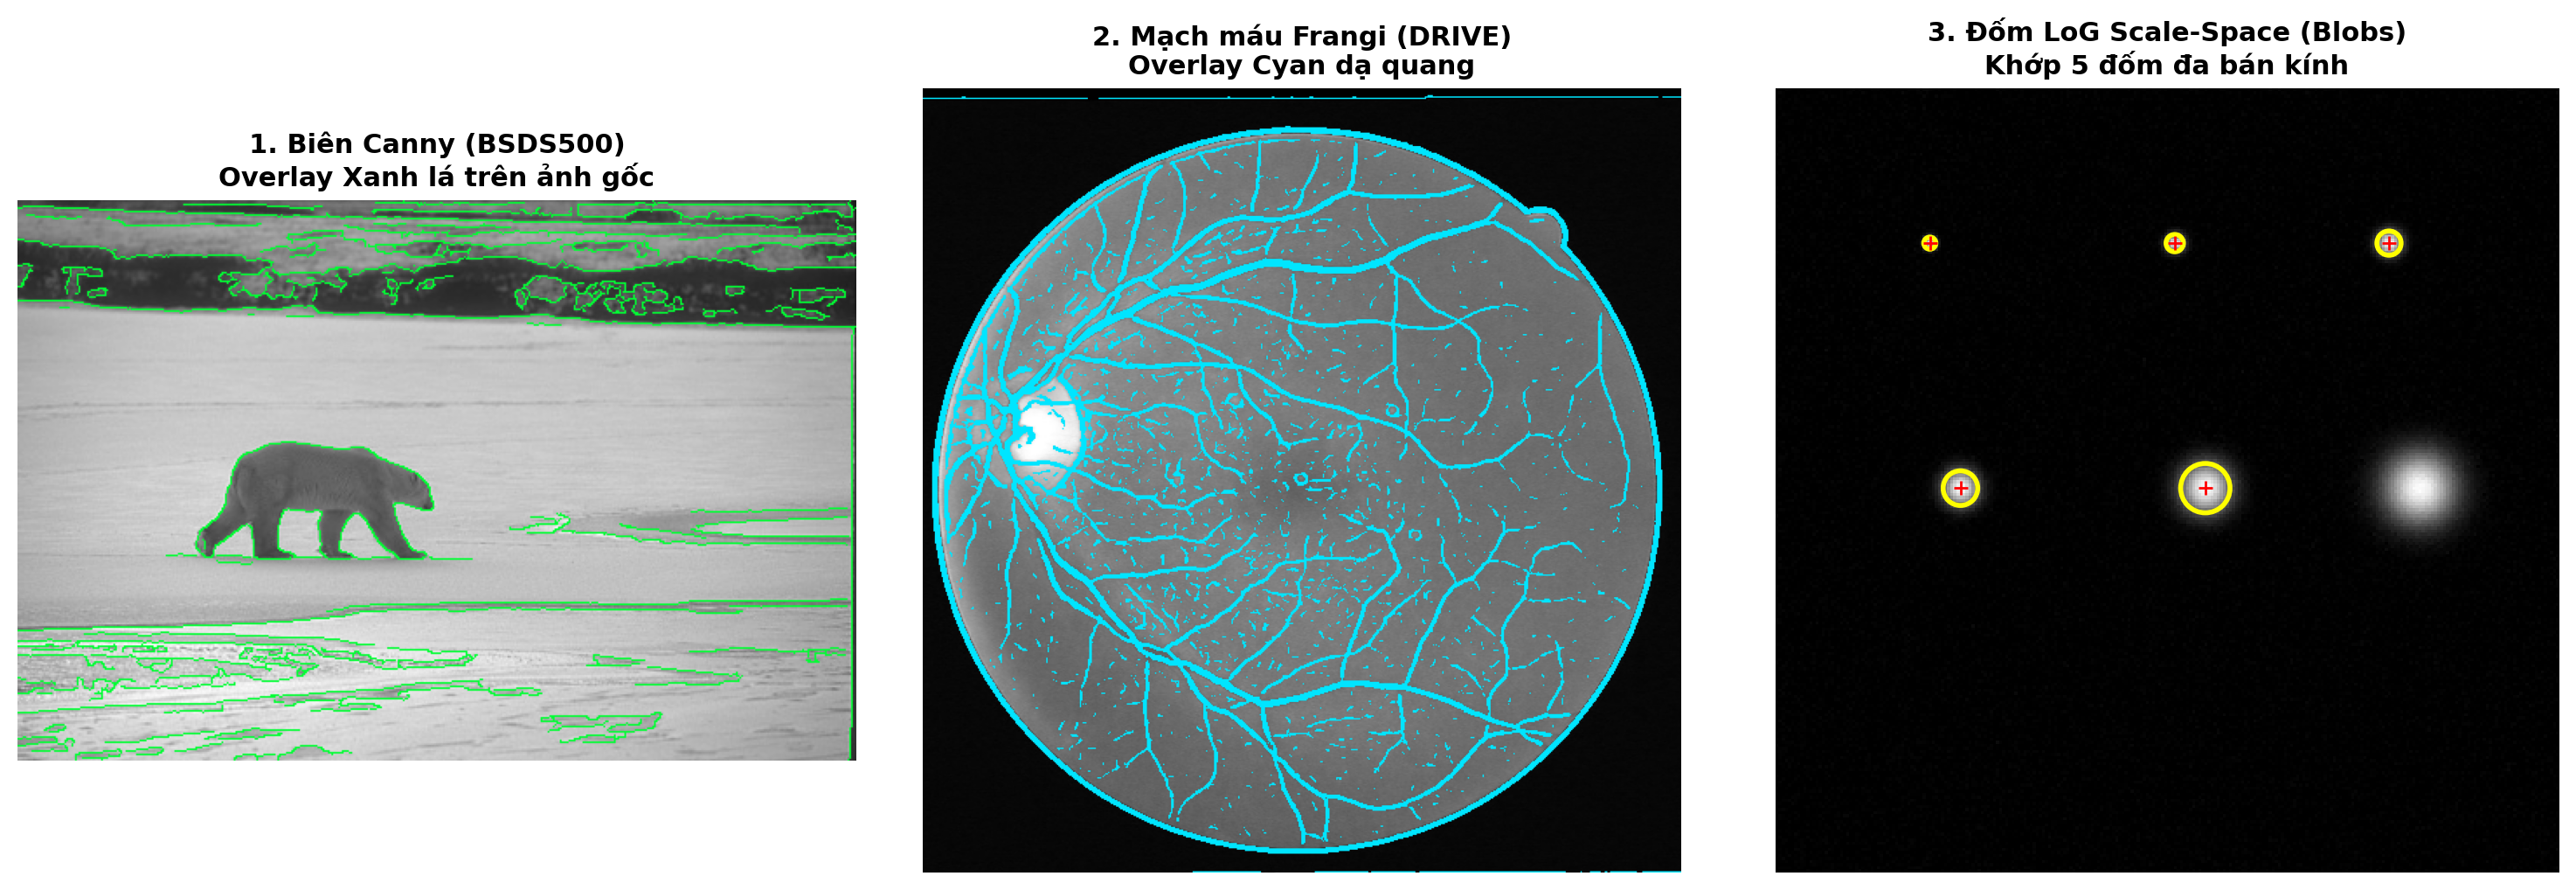
\includegraphics[width=0.95\textwidth]{figures/showcase_detector_overlays.png}
\caption{Minh họa kết quả thực thi của 3 bộ phát hiện đặc trưng mức cao trên hệ thống Python Core: (a) Canny Edge Detection trên ảnh tự nhiên BSDS500; (b) Frangi Vesselness Filter trên ảnh đáy mắt DRIVE; (c) LoG Blob Detection trên ảnh tế bào sinh học hiển vi.}
\label{fig:detector_overlays}
\end{figure*}

\subsection{Chiến Lược Tối Ưu Hóa và Phân Tích Độ Phức Tạp Thuật Toán}
\subsubsection{Vector hóa toàn phần bằng NumPy (Array Broadcasting)}
Để đạt được hiệu năng tiệm cận các thư viện viết bằng C/C++, hệ thống loại bỏ triệt để các vòng lặp lồng nhau qua tọa độ từng pixel ($y, x$). Tất cả các phép toán tính trị riêng ma trận Hessian, tính chỉ số Frangi, so sánh ngưỡng NMS đều được biểu diễn dưới dạng biểu thức mảng phát thanh đa chiều. Thư viện NumPy tự động biên dịch các biểu thức này thành các tập lệnh tối ưu vector SIMD (AVX2 / AVX-512) trên phần cứng CPU hiện đại.

\subsubsection{Quản lý độ chính xác số học và Bộ nhớ}
Quá trình tính toán trung gian được duy trì ở kiểu số thực dấu chấm động độ chính xác kép \texttt{float64} (64-bit). Điều này ngăn ngừa sai số tích lũy từ các phép nhân dồn và phép trừ ma trận có độ lệch giá trị nhỏ. Chỉ tại bước cuối cùng khi xuất file ảnh lưu trữ đĩa (TIFF 32-bit), dữ liệu mới được ép kiểu an toàn sang \texttt{float32}.

\subsubsection{Bảng tổng hợp độ phức tạp thuật toán}
\begin{table}[htbp]
\caption{Độ phức tạp thời gian và không gian của các mô-đun lõi}
\centering
\begin{tabular}{lcc}
\toprule
\textbf{Mô-đun / Thuật toán} & \textbf{Độ phức tạp thời gian} & \textbf{Độ phức tạp bộ nhớ} \\
\midrule
Gaussian Smoothing 1D & $\mathcal{O}(2K \cdot HW)$ & $\mathcal{O}(HW)$ \\
Gradient Vector $(\|\nabla L\|, \theta)$ & $\mathcal{O}(2K \cdot HW)$ & $\mathcal{O}(HW)$ \\
Ma trận Hessian \& Trị riêng & $\mathcal{O}(6K \cdot HW)$ & $\mathcal{O}(HW)$ \\
Structure Tensor $(\sigma_d, \sigma_i)$ & $\mathcal{O}((4K_d + 3K_i) \cdot HW)$ & $\mathcal{O}(HW)$ \\
Canny NMS \& Hysteresis BFS & $\mathcal{O}(HW)$ & $\mathcal{O}(HW)$ \\
Frangi Filter ($|\Sigma|$ tỷ lệ) & $\mathcal{O}(|\Sigma| \cdot 6K \cdot HW)$ & $\mathcal{O}(HW)$ \\
LoG Extrema 3D ($|\Sigma|$ tỷ lệ) & $\mathcal{O}(|\Sigma| \cdot HW)$ & $\mathcal{O}(|\Sigma| \cdot HW)$ \\
\bottomrule
\end{tabular}
\label{tab:complexity}
\end{table}



% BEGIN AUTO_CH5
\section{Chương 5: Thực Nghiệm, Đánh Giá Định Lượng và Phân Tích}
\subsection{Dữ liệu và protocol có thể tái lập}
Bộ dữ liệu gồm 25 ảnh xám uint8: 10 BSDS500 với 56 bộ nhãn đa annotator, 10 DRIVE có vessel mask/FOV, 4 ảnh blob tổng hợp và ảnh tế bào \texttt{blob\_05}. Ảnh tế bào có 276 đối tượng và 15 vùng loại trừ, được nhóm xây dựng và Đức rà soát; không coi là nhãn chuyên gia độc lập.
Nguồn chính của chương này là \texttt{outputs/metrics/duc\_10\_11} và \texttt{outputs/analysis/duc\_task5\_10\_11}, kèm manifest SHA-256. Checksum xác minh toàn vẹn từng bộ, không chứng minh Python và Fiji có cùng byte hoặc cùng giá trị số.

\subsection{Tầng 1: đối chuẩn bản đồ liên tục}
Đối chiếu 220 cặp TIFF trên năm ảnh đại diện, crop theo support của từng toán tử. Ngưỡng gốc yêu cầu đồng thời relative max error $<10^{-4}$ và Pearson $r>0.9999$. Có 35 cặp đạt ngưỡng gốc và 185 cặp chưa đạt. Nếu nhóm dùng ngưỡng mở rộng $10^{-2}$, cần ghi rõ 185 cặp là RELAXED, không phải STRICT. PSNR với MAX=255 chỉ áp dụng Gaussian; đạo hàm có dấu dùng MAE/RMSE/relative error/Pearson. Tương quan cao không đủ chứng minh tương đương biên độ. Khác biệt rời rạc hóa là giả thuyết cần đối chiếu hồ sơ hiệu chuẩn.

\subsection{Tầng 2: biên BSDS500}
Dung sai là đĩa Euclidean bán kính 2 px. Precision xét biên của ít nhất một annotator; recall trung bình các annotator. Ngưỡng phân vị tính trên NMS khác 0, chọn lưới thô/tinh riêng từng sigma trên Python rồi đóng băng cho Fiji. Ảnh NMS rỗng vẫn được tính vào mẫu số. FeatureJ Edges dùng Canny với NMS nội suy và hysteresis, là nhánh tham chiếu riêng, không phải zero-crossing Laplacian.
\begin{table}[htbp]\centering
\caption{F1 trung bình trên 10 ảnh BSDS; cùng ngưỡng cho hai nguồn}\label{tab:duc10_bsds}
\begin{tabular}{rrrr}\toprule
$\sigma$ & Python & Fiji & Fiji--Python \\\midrule
1 & 0.455418 & 0.455478 & +0.00006020 \\
2 & 0.477886 & 0.477886 & +0.00000000 \\
4 & 0.441491 & 0.441491 & +0.00000000 \\
8 & 0.343340 & 0.343340 & +0.00000000 \\
\bottomrule\end{tabular}\end{table}

\subsection{Tầng 2: ridge và blob}
DRIVE lấy cực đại Frangi qua các scale đã chuẩn hóa. Vùng đánh giá là giao các FOV hợp lệ qua scale, với support lấy từ config (hiện 32 px); ngưỡng tuyệt đối được chọn trong lưới đã công bố trên Python và dùng chung cho Fiji. Vì khác vùng FOV/ngưỡng, không so trực tiếp điểm này với phiên cũ dùng FOV 8 px hoặc phân vị p85.
Blob dùng đúng 7 sigma config cho cả hai nguồn, ghép một--một theo maximum cardinality với tâm lệch $\le2$ px và bán kính sai $\le20\%$. Bỏ dự đoán có tâm trong vùng ignore trước khi tính FP.
\begin{table}[htbp]\centering\small
\caption{Macro Precision/Recall/F1 của ridge và blob}\label{tab:duc10_accuracy}
\begin{tabular}{lrrr}\toprule
Nguồn / bài toán & P & R & F1 \\\midrule
python / ridge\_drive & 0.811157 & 0.352088 & 0.477382 \\
python / blob\_log & 0.895563 & 0.901449 & 0.898418 \\
fiji / ridge\_drive & 0.814269 & 0.347986 & 0.473863 \\
fiji / blob\_log & 0.894237 & 0.900725 & 0.897373 \\
\bottomrule\end{tabular}\end{table}
\begin{table}[htbp]\centering
\caption{Ảnh tế bào: GT=276; dự đoán sau ignore; số bỏ qua}\label{tab:duc10_cells}
\begin{tabular}{lrrrr}\toprule
Nguồn & TP & Dự đoán & Ignore & F1 \\\midrule
python & 140 & 293 & 36 & 0.492091 \\
fiji & 139 & 295 & 37 & 0.486865 \\
\bottomrule\end{tabular}\end{table}
Macro đặt mỗi ảnh cùng trọng số; micro gộp số đối tượng. Bốn ảnh tổng hợp dễ có ảnh hưởng lớn đến macro nên cần báo cáo cả hai. python: macro F1=0.898418, micro F1=0.519135; fiji: macro F1=0.897373, micro F1=0.514096. Audit từng cặp được lưu đầy đủ trong CSV/JSON của phiên chạy.

\subsection{Biểu đồ và thời gian thực thi}
357 trường hợp mỗi nguồn được đo một warm-up và năm lượt đo, lấy median, giữ mẫu thô và fingerprint code/config/raw. Java đo API ImageScience headless, không gồm GUI hay đọc/ghi TIFF; không tuyên bố hai engine có precision nội bộ giống nhau hoặc ưu thế tốc độ trên mọi máy.
\begin{figure}[htbp]\centering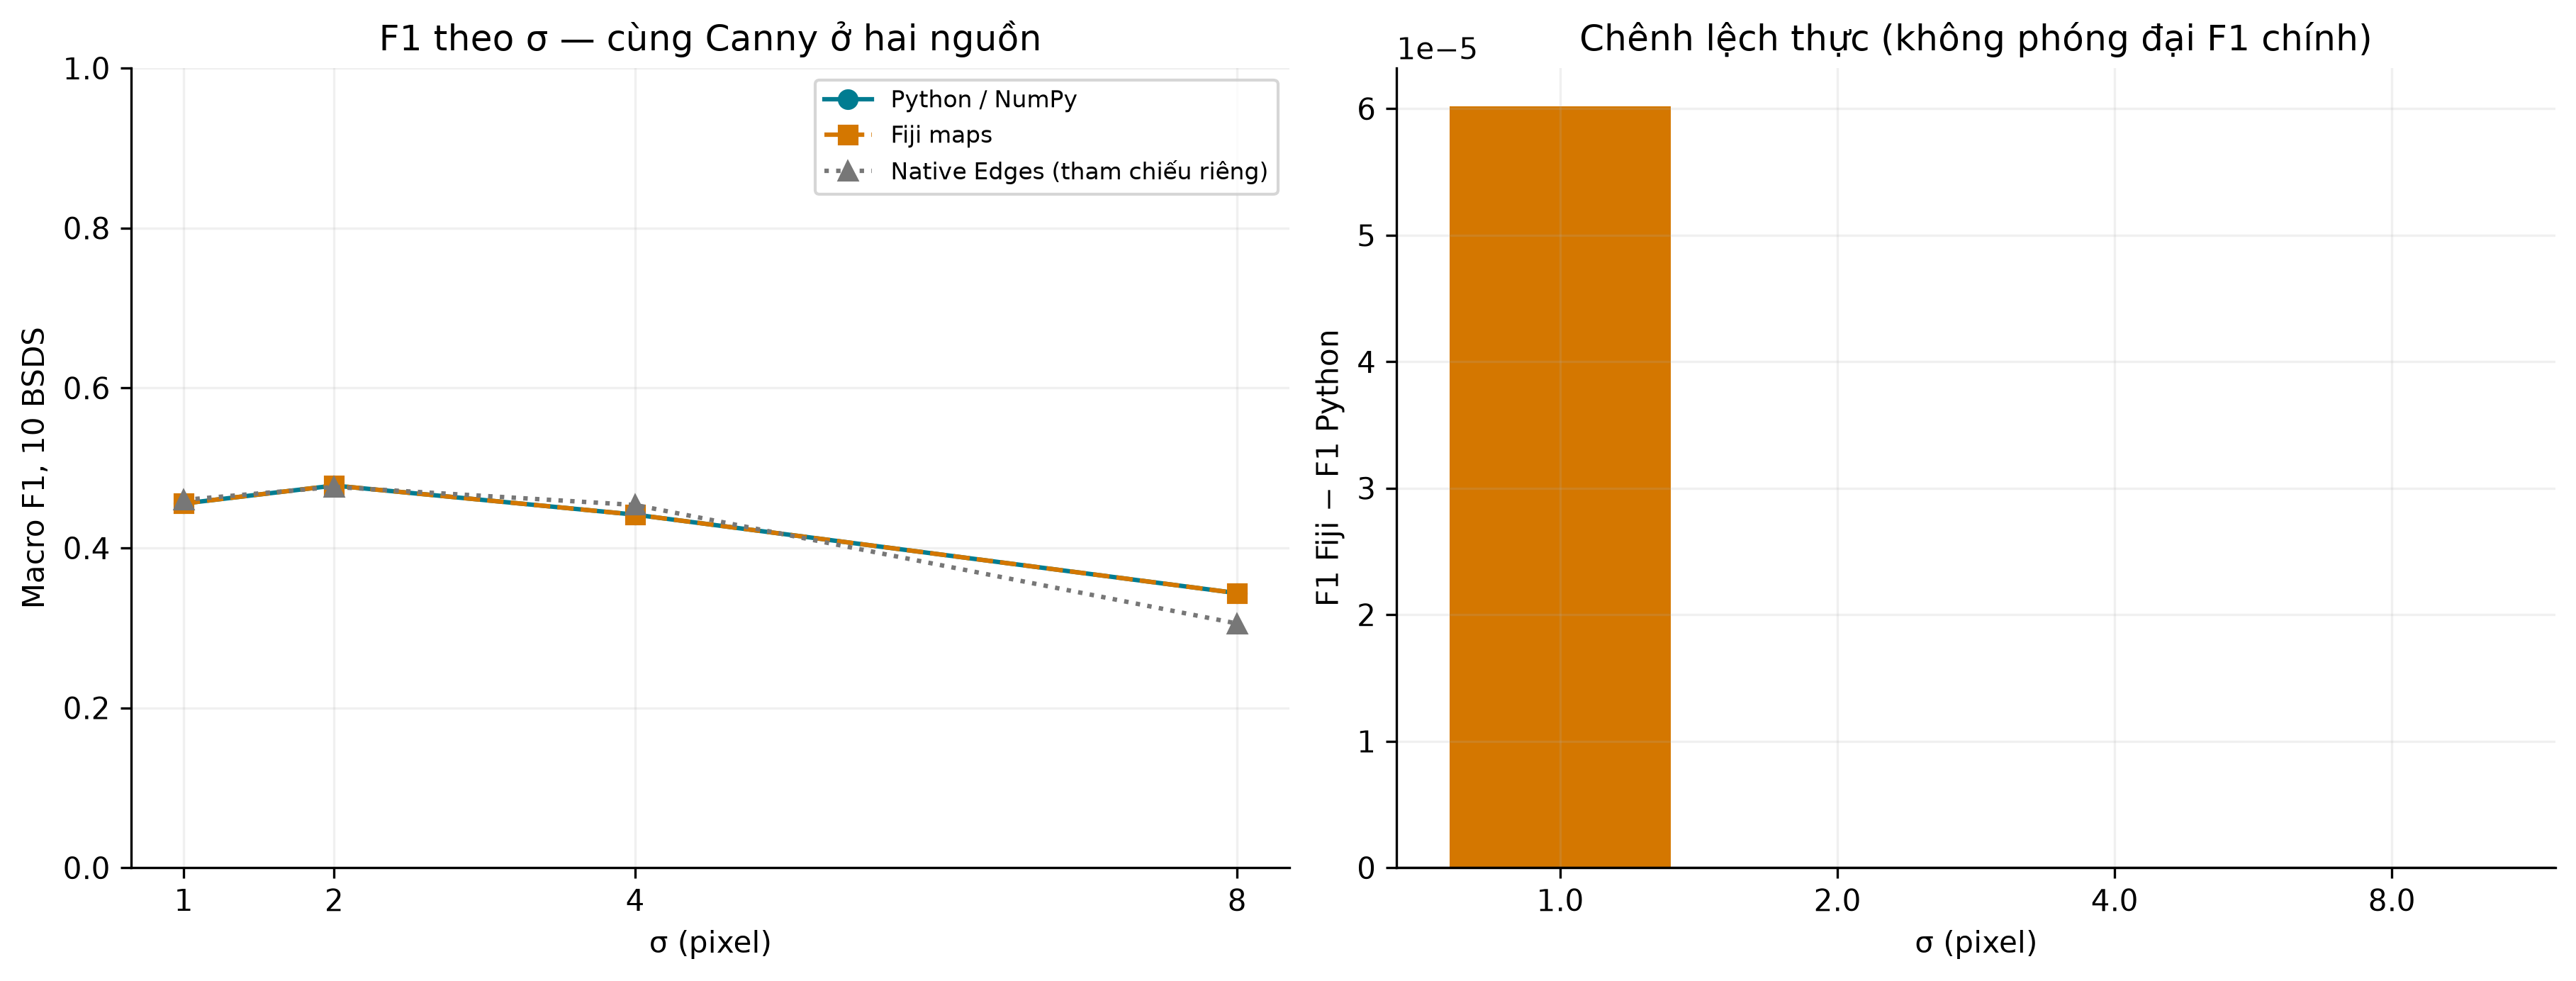
\includegraphics[width=\linewidth]{figures/duc10_04_f1_theo_sigma.png}\caption{F1 theo sigma trên cùng protocol.}\end{figure}
\begin{figure}[htbp]\centering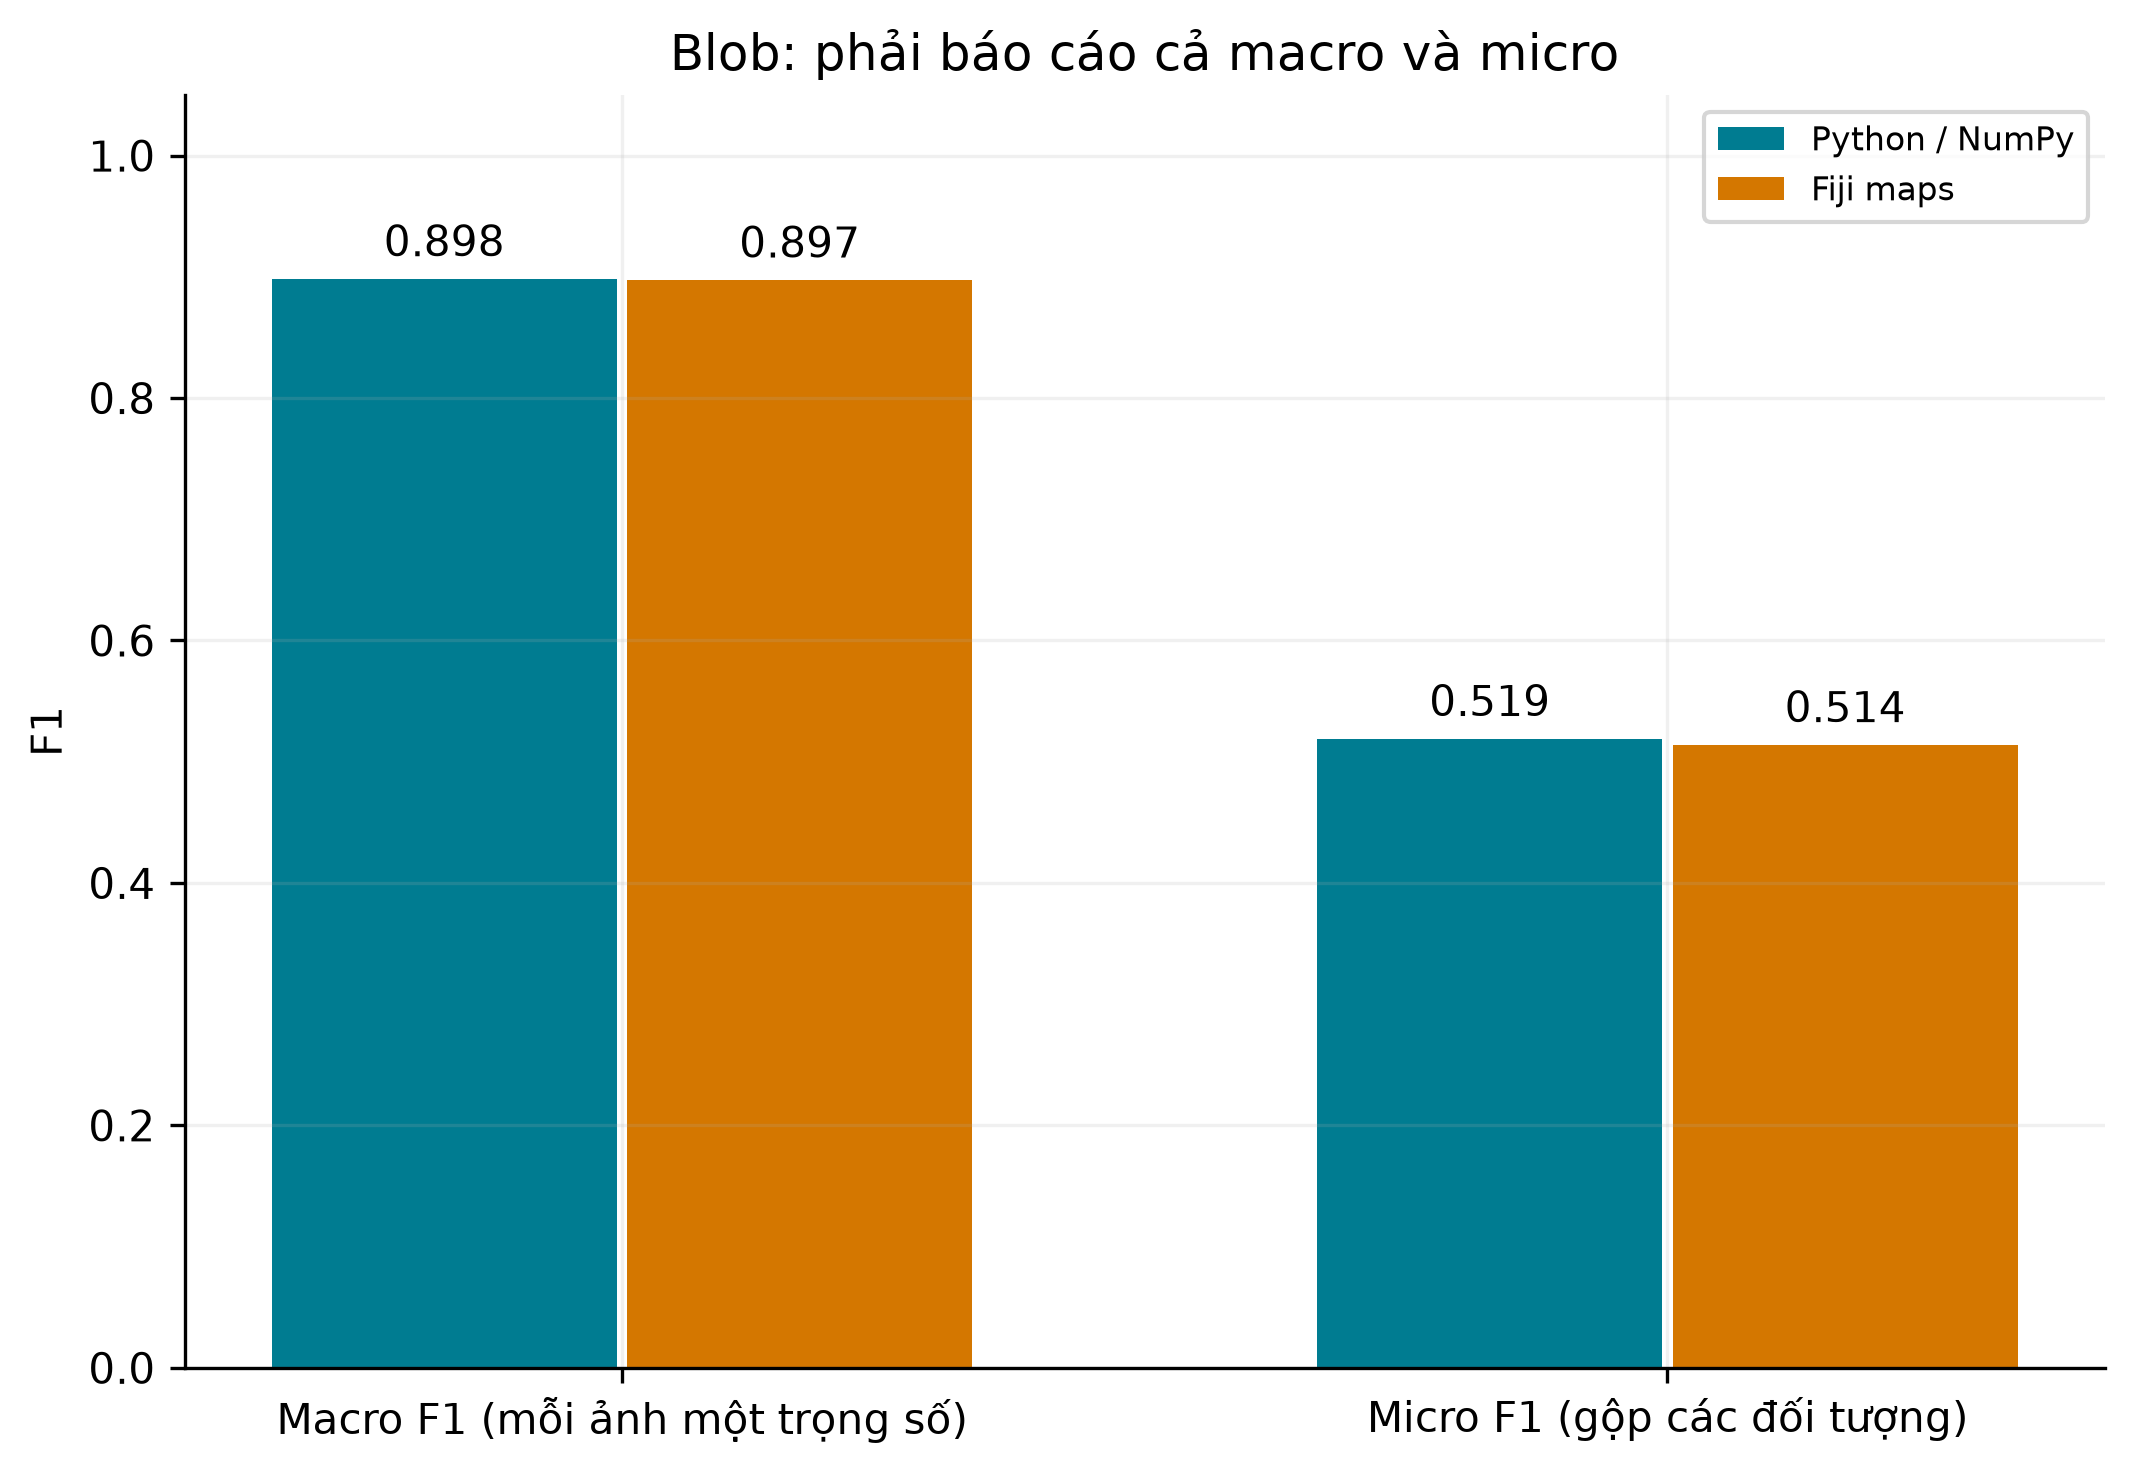
\includegraphics[width=\linewidth]{figures/duc10_08_blob_macro_micro.png}\caption{Macro/micro F1 trên tập blob.}\end{figure}
\begin{figure}[htbp]\centering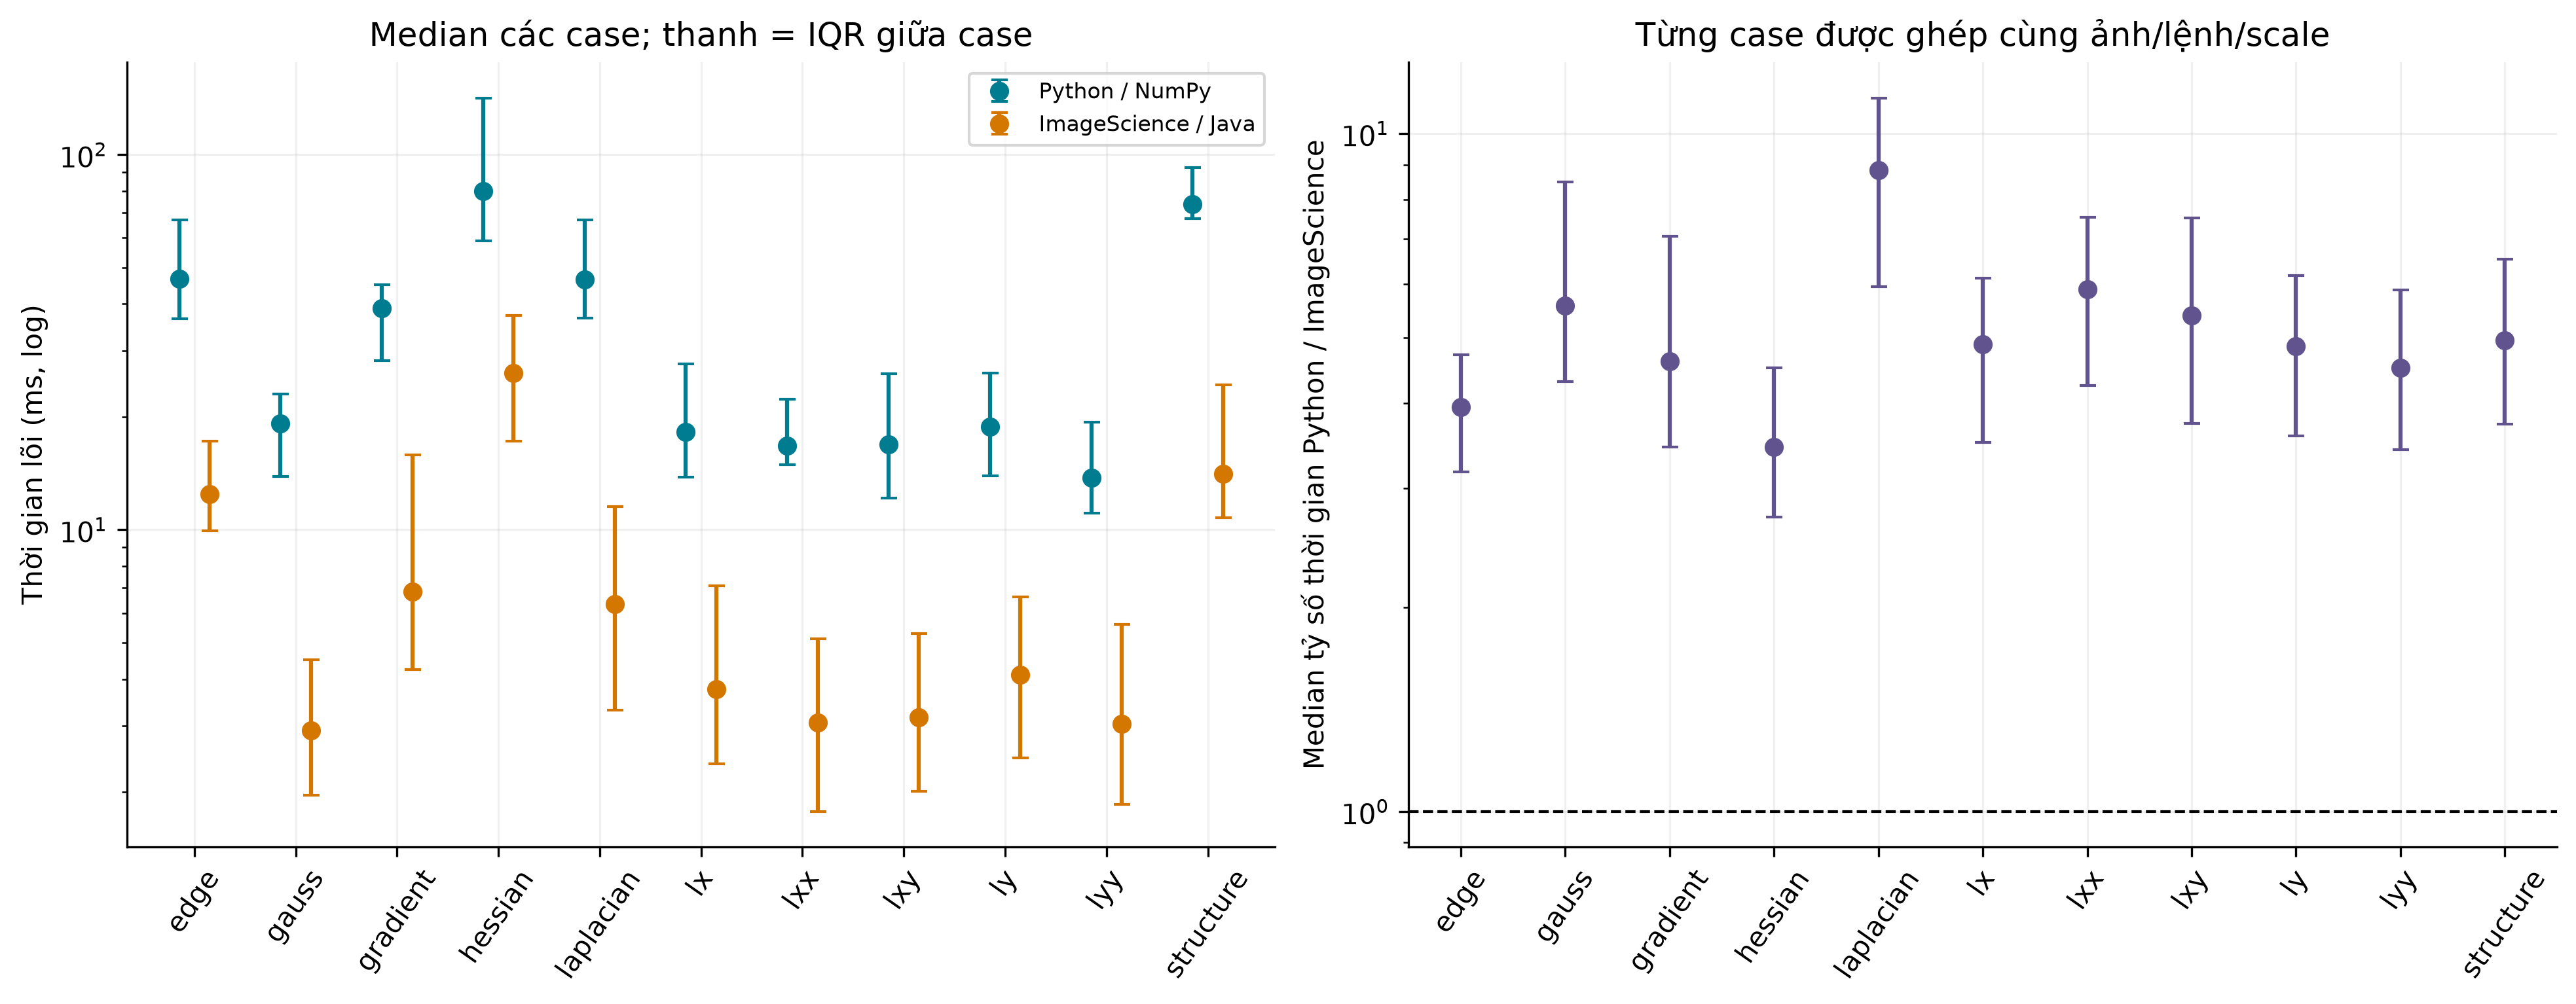
\includegraphics[width=\linewidth]{figures/duc10_09_thoi_gian_theo_lenh.png}\caption{Median thời gian theo lệnh; API headless, không gồm I/O.}\end{figure}

\subsection{Giới hạn}
Ngưỡng được chọn và đánh giá trên cùng tập nội bộ, không phải điểm test độc lập của benchmark chính thức. Chưa chạy biến thể nhiễu/kích thước; không kết luận độ bền với nhiễu. Nhãn tế bào do nhóm rà soát; trường hợp dính/cắt biên được loại theo vùng ignore. Detector LoG hiện bỏ hai đầu lưới scale, nên đối tượng ngoài dải vẫn có thể làm giảm recall.
% END AUTO_CH5

% BEGIN AUTO_CH6
\section{Chương 6: Kết Luận và Hướng Phát Triển}
Nhóm đã hiện thực Gaussian, đạo hàm bậc 1/2, gradient, Hessian, Canny, Frangi, LoG và Structure Tensor bằng NumPy; kiểm thử và đánh giá trên hai nguồn bản đồ cùng hậu xử lý. Kết quả số học chưa đạt ngưỡng gốc cho mọi cặp; giữ rõ STRICT và RELAXED. Đánh giá GT áp dụng matching một--một, ignore và cùng cấu hình cho hai nguồn. Công việc tiếp theo là kiểm chứng hiệu chuẩn, mở rộng dữ liệu/tập tách biệt và thực nghiệm nhiễu trước khi đưa ra kết luận khái quát.
% END AUTO_CH6

\bibliographystyle{IEEEtran}
\bibliography{references}

\end{document}
